\section{4L Neural Network}
A \textbf{4-Layer Neural Network (4L)} extends the 2L architecture by adding two hidden layers between the input and output layers (input $\rightarrow$ hidden 1 $\rightarrow$ hidden 2 $\rightarrow$ output). Each hidden layer applies a linear transformation followed by a nonlinear activation function, which allows the network to learn nonlinear relationships and interactions between the predictor variables. The output layer uses the identity activation, as is standard for regression.
\medskip

For this project, the 4L Neural Network is implemented using \textbf{PyTorch} to perform regression on the same three datasets: Airfoil Self-Noise, Auto MPG, and Concrete Compressive Strength. The goal is to evaluate its predictive performance through hyperparameter tuning and Quality of Fit (QoF) measures, including R², MSE, and RMSE, for both in-sample and validation data, and to compare it with the PyTorch 2L Neural Network.

\subsection{PyTorch}
Each dataset was split into 80\% training and 20\% validation data using the same random seed as the PyTorch 2L model, so both models are evaluated on identical observations. The predictors were standardized using training data statistics. Unlike the 2L model, the target variable was also standardized using the training mean and standard deviation, since networks with hidden layers train poorly when the target is on a large raw scale (e.g., about 125 dB for Airfoil). All predictions were converted back to the original scale before calculating the QoF measures, so the MSE and RMSE values are directly comparable with the 2L results.
\medskip

Hyperparameter tuning was performed with a grid search over the number of nodes in the two hidden layers $\{(16, 8), (32, 16), (64, 32), (128, 64)\}$, the activation function $\{$ReLU, Tanh, Sigmoid$\}$, the mini-batch size $\{16, 32, 64\}$, and the learning rate $\{0.001, 0.005, 0.01, 0.05\}$, giving 144 configurations per dataset. Each configuration was trained with the Adam optimizer for a maximum of 300 epochs with early stopping (patience = 20), using an inner 80/20 split of the training data, so the 20\% validation set was never used during tuning. The final model for each dataset was then retrained on the full training set for the best number of epochs found during tuning.
\medskip
\begin{table}[H]
    \centering
    \caption{PyTorch 4L Neural Network Hyperparameter Tuning Results}
    \label{tab:pytorch4l_hyperparameters}
    \small
    \begin{tabular}{lcccccc}
        \hline
        \textbf{Dataset} & \textbf{Hidden Nodes} & \textbf{Activation} & \textbf{Learning Rate} & \textbf{Batch Size} & \textbf{Validation MSE} & \textbf{Best Epoch} \\
        \hline
        Airfoil  & (128, 64) & ReLU & 0.001 & 16 & 3.0190 & 225 \\
        Auto MPG & (64, 32) & Tanh & 0.050 & 32 & 5.9313 & 14 \\
        Concrete & (64, 32) & ReLU & 0.005 & 64 & 15.8281 & 86 \\
        \hline
    \end{tabular}
\end{table}

As shown in Table \ref{tab:pytorch4l_hyperparameters}, the selected hyperparameters differ across datasets. ReLU was selected for Airfoil and Concrete, while Tanh was selected for Auto MPG. Airfoil selected the largest network (128 and 64 nodes) with the smallest learning rate (0.001), which required 225 epochs to reach its best validation loss. Since this configuration lies on the edge of the search space, a larger network or smaller learning rate may improve Airfoil further. Auto MPG reached its best validation loss after only 14 epochs with a high learning rate of 0.05, which reflects its small size (250 tuning observations). The tuning validation MSE values are much lower than those of the 2L model (Table \ref{tab:pytorch_hyperparameters}), e.g., 3.02 vs. 31.51 for Airfoil and 15.83 vs. 106.18 for Concrete.
\medskip
\begin{figure}[H]
    \centering
    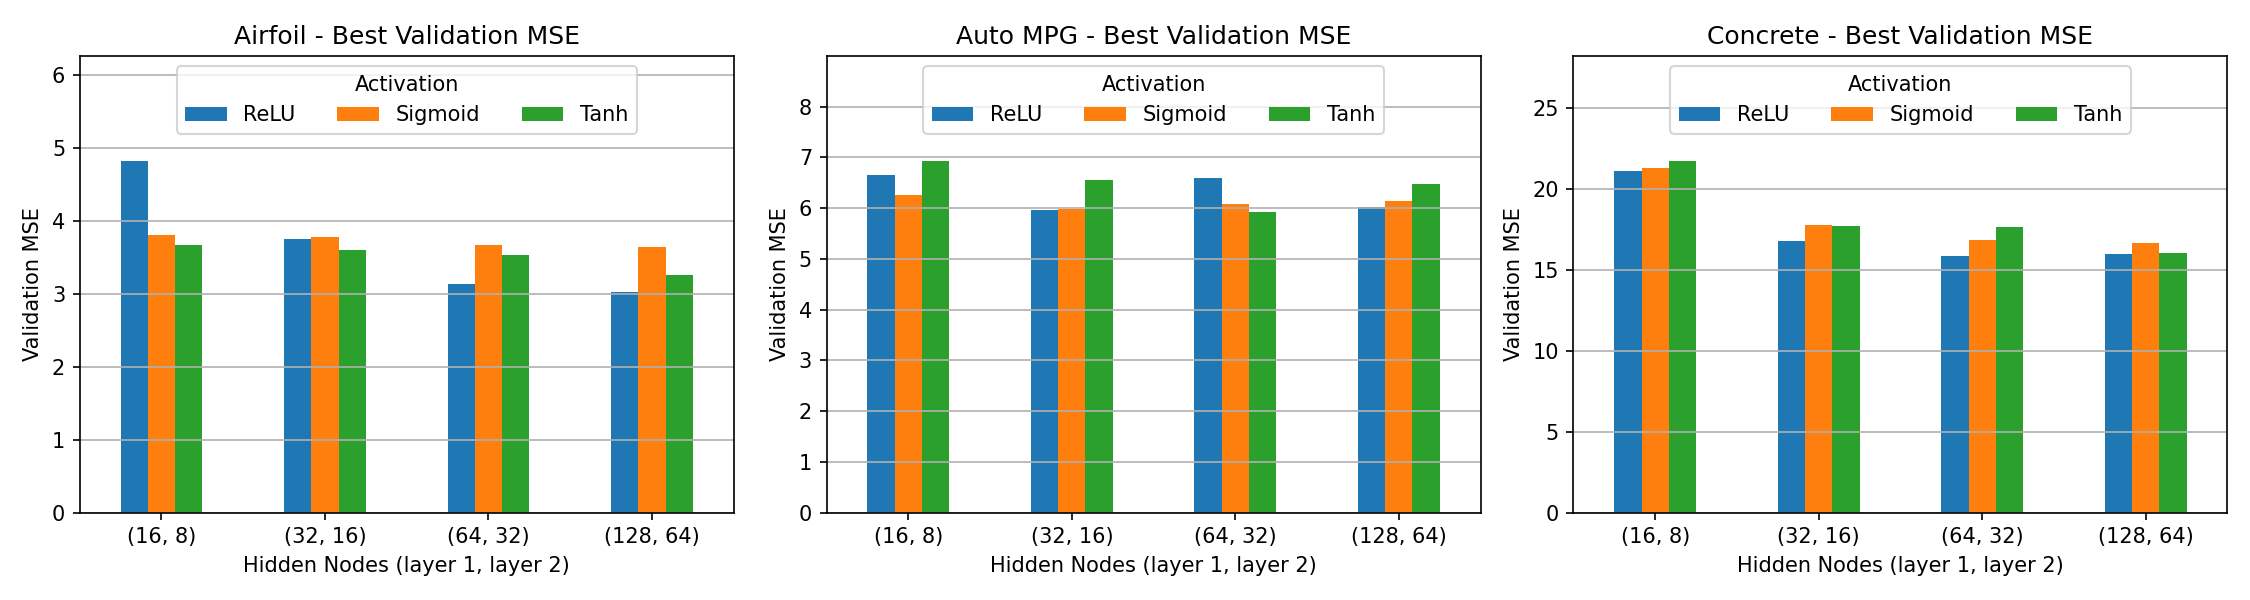
\includegraphics[width=\linewidth]{4L/tuning_sensitivity.png}
    \caption{PyTorch 4L Best Tuning Validation MSE by Hidden Layer Size and Activation Function}
    \label{fig:pytorch4l_tuning}
\end{figure}

Figure \ref{fig:pytorch4l_tuning} shows the best tuning validation MSE for each hidden layer size and activation function. For Airfoil and Concrete, the validation MSE generally decreases as the number of hidden nodes increases: the smallest network (16, 8) performs worst on both datasets, and ReLU performs best for the larger networks. For Concrete, the largest improvement occurs between (16, 8) and (32, 16), while Airfoil continues to improve up to (128, 64). For Auto MPG, the differences across sizes and activation functions are small (about 5.9 to 6.9), suggesting that its relationships are simple enough that network size has little effect.
\medskip
\begin{table}[H]
    \centering
    \caption{PyTorch 4L Neural Network Quality of Fit Results}
    \label{tab:pytorch4l_qof}
    \small
    \resizebox{\textwidth}{!}{
    \begin{tabular}{lcccccc}
        \hline
        \textbf{Dataset} & \textbf{Train $R^2$} & \textbf{Validation $R^2$} & \textbf{Train MSE} & \textbf{Validation MSE} & \textbf{Train RMSE} & \textbf{Validation RMSE} \\
        \hline
        Airfoil  & 0.9720 & 0.9643 & 1.3152 & 1.7895 & 1.1468 & 1.3377 \\
        Auto MPG & 0.8581 & 0.8317 & 8.9528 & 8.5903 & 2.9921 & 2.9309 \\
        Concrete & 0.9623 & 0.8691 & 10.6965 & 33.7271 & 3.2706 & 5.8075 \\
        \hline
    \end{tabular}
    }
\end{table}

The Quality of Fit (QoF) results were evaluated using R², MSE, and RMSE for both in-sample (training) and validation data. As shown in Table \ref{tab:pytorch4l_qof}, Airfoil achieved the highest validation R² of 0.9643, followed by Concrete at 0.8691 and Auto MPG at 0.8317. Airfoil's training and validation R² values are very close, indicating that the model generalizes well. Concrete shows the largest gap between training (0.9623) and validation (0.8691) R², and its validation MSE (33.73) is about three times its training MSE (10.70), indicating some overfitting. Auto MPG shows a small gap, and its validation MSE is slightly lower than its training MSE, which can occur with a small validation set of 79 observations. To check that these results do not depend on a single random initialization, the final models were retrained with five different seeds. The mean validation R² values were 0.9610 ($\pm$0.0082) for Airfoil, 0.8525 ($\pm$0.0255) for Auto MPG, and 0.8738 ($\pm$0.0111) for Concrete, consistent with Table \ref{tab:pytorch4l_qof}.
\medskip
\begin{figure}[H]
    \centering

    \begin{minipage}{0.32\textwidth}
        \centering
        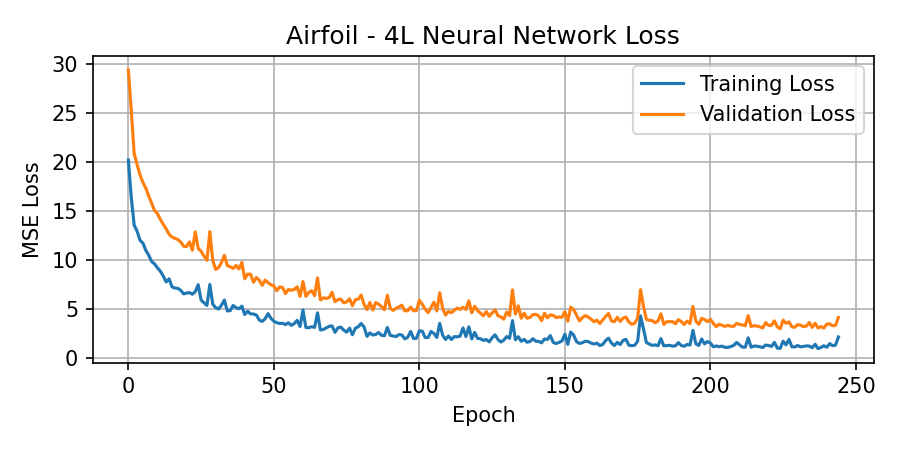
\includegraphics[width=\linewidth]{4L/airfoil_loss.png}
        \small (a) Airfoil
    \end{minipage}
    \hfill
    \begin{minipage}{0.32\textwidth}
        \centering
        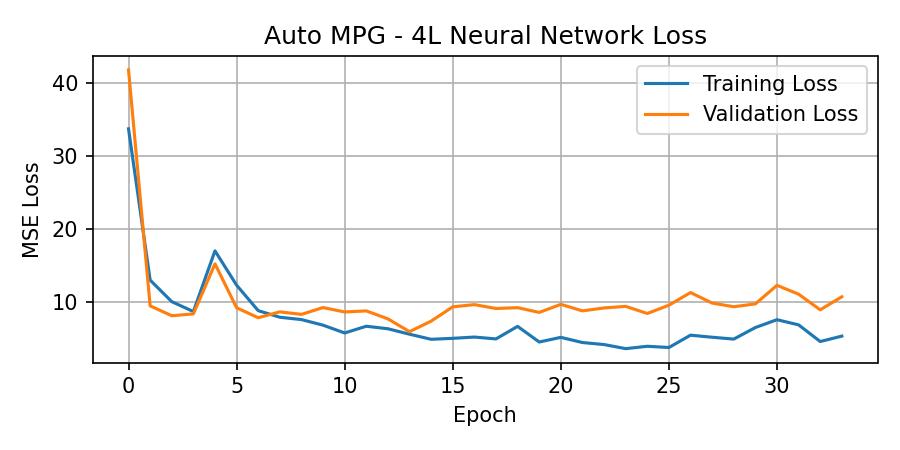
\includegraphics[width=\linewidth]{4L/autompg_loss.png}
        \small (b) Auto MPG
    \end{minipage}
    \hfill
    \begin{minipage}{0.32\textwidth}
        \centering
        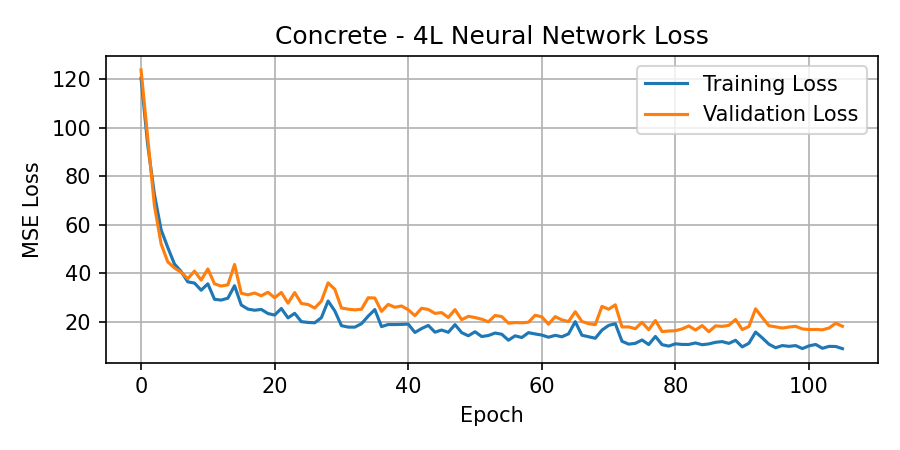
\includegraphics[width=\linewidth]{4L/concrete_loss.png}
        \small (c) Concrete
    \end{minipage}

    \caption{PyTorch 4L Neural Network Training and Validation Loss vs. Epoch}
    \label{fig:pytorch4l_loss}
\end{figure}

Figure \ref{fig:pytorch4l_loss} shows the training and validation loss vs epoch plots for the best configuration of each dataset. Airfoil shows a steady decrease in both losses over about 225 epochs, with the validation loss remaining close to the training loss. Auto MPG drops sharply within the first few epochs and reaches its best validation loss at epoch 14; after that, the training loss keeps decreasing while the validation loss slowly rises, which is an early sign of overfitting that early stopping prevents. Concrete decreases steadily, but the gap between the training and validation losses widens after roughly 70 epochs, consistent with its larger training--validation gap in Table \ref{tab:pytorch4l_qof}. Compared with the 2L loss curves (Figure \ref{fig:pytorch_loss}), the 4L curves are noisier, which is expected from the larger number of parameters and the use of mini-batches.
\medskip
\begin{figure}[H]
    \centering

    \begin{minipage}{0.32\textwidth}
        \centering
        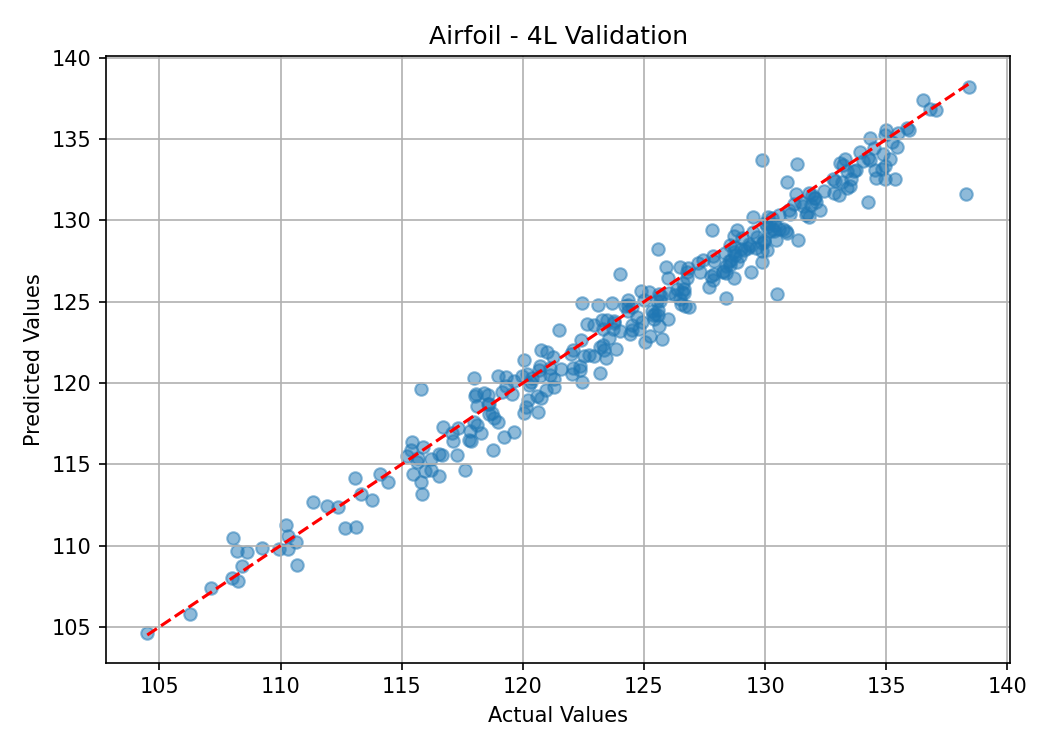
\includegraphics[width=\linewidth]{4L/airfoil_actual.png}
        \small (a) Airfoil
    \end{minipage}
    \hfill
    \begin{minipage}{0.32\textwidth}
        \centering
        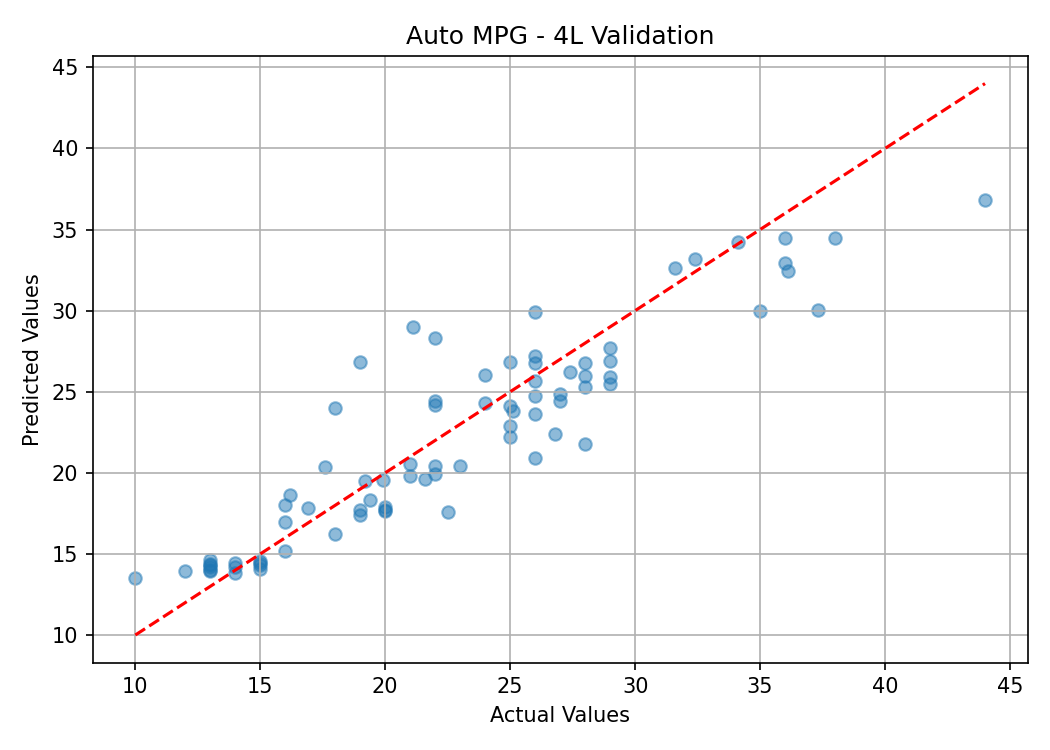
\includegraphics[width=\linewidth]{4L/autompg_actual.png}
        \small (b) Auto MPG
    \end{minipage}
    \hfill
    \begin{minipage}{0.32\textwidth}
        \centering
        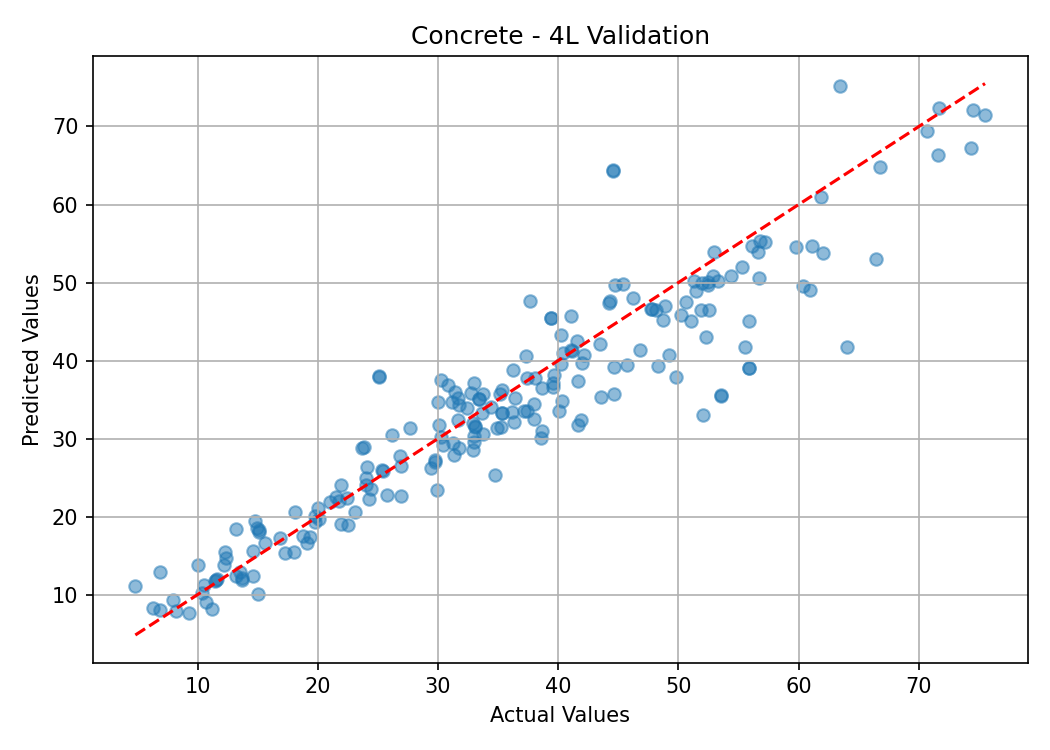
\includegraphics[width=\linewidth]{4L/concrete_actual.png}
        \small (c) Concrete
    \end{minipage}

    \caption{PyTorch 4L Neural Network Validation Actual vs. Predicted Values}
    \label{fig:pytorch4l_actual}
\end{figure}

Figure \ref{fig:pytorch4l_actual} shows the validation actual vs predicted plots for the three datasets. The red dashed diagonal line represents perfect predictions. Airfoil's points lie tightly along the diagonal line across the full range of sound pressure levels, a large improvement over the 2L model (Figure \ref{fig:pytorch_actual}). Concrete also follows the diagonal closely, with more spread at mid-range strengths (30--55 MPa). Auto MPG follows the diagonal for most observations but underestimates the highest-mpg cars (e.g., an actual value of 44 mpg is predicted at about 37 mpg).
\medskip
\begin{figure}[H]
    \centering

    \begin{minipage}{0.32\textwidth}
        \centering
        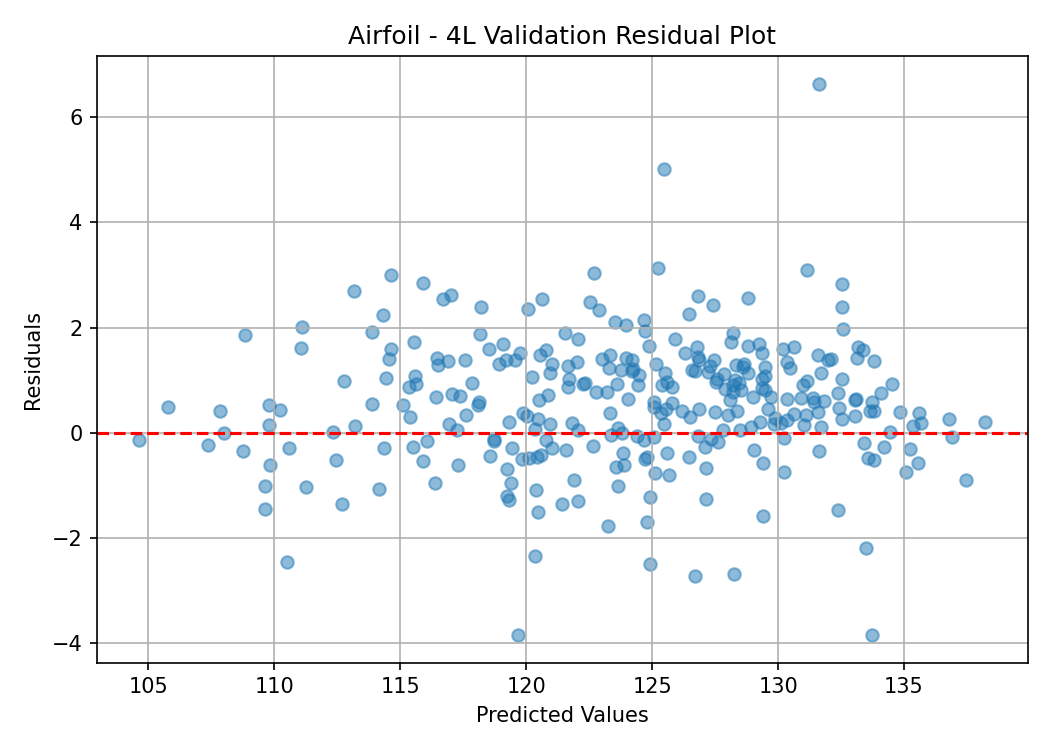
\includegraphics[width=\linewidth]{4L/airfoil_residual.png}
        \small (a) Airfoil
    \end{minipage}
    \hfill
    \begin{minipage}{0.32\textwidth}
        \centering
        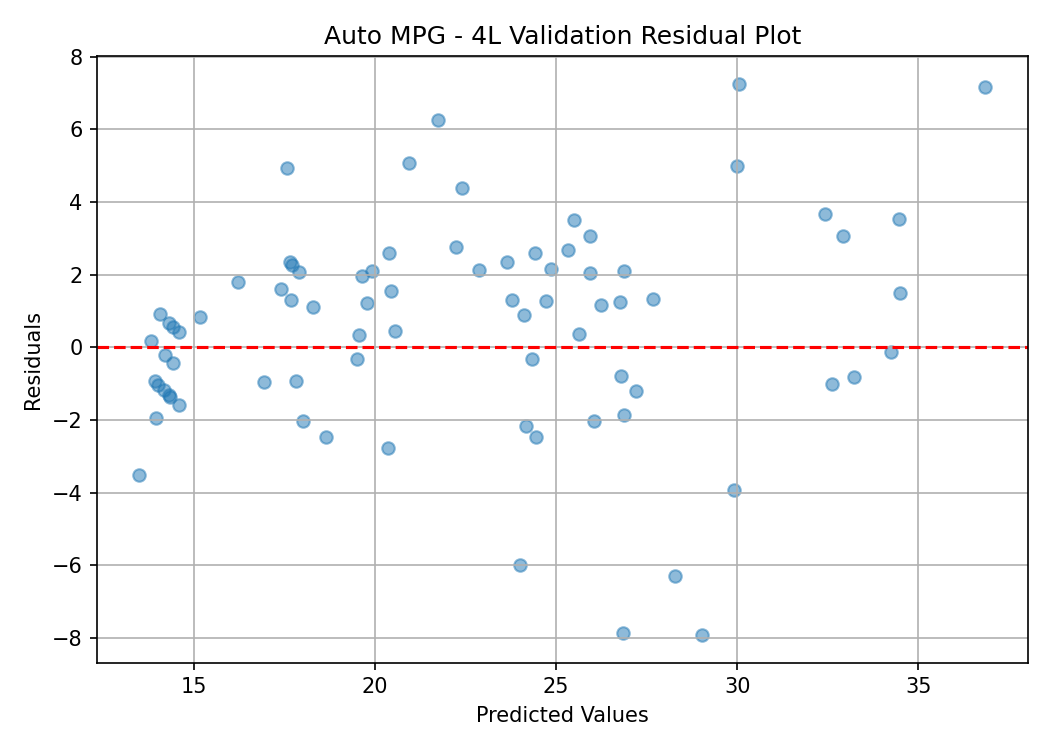
\includegraphics[width=\linewidth]{4L/autompg_residual.png}
        \small (b) Auto MPG
    \end{minipage}
    \hfill
    \begin{minipage}{0.32\textwidth}
        \centering
        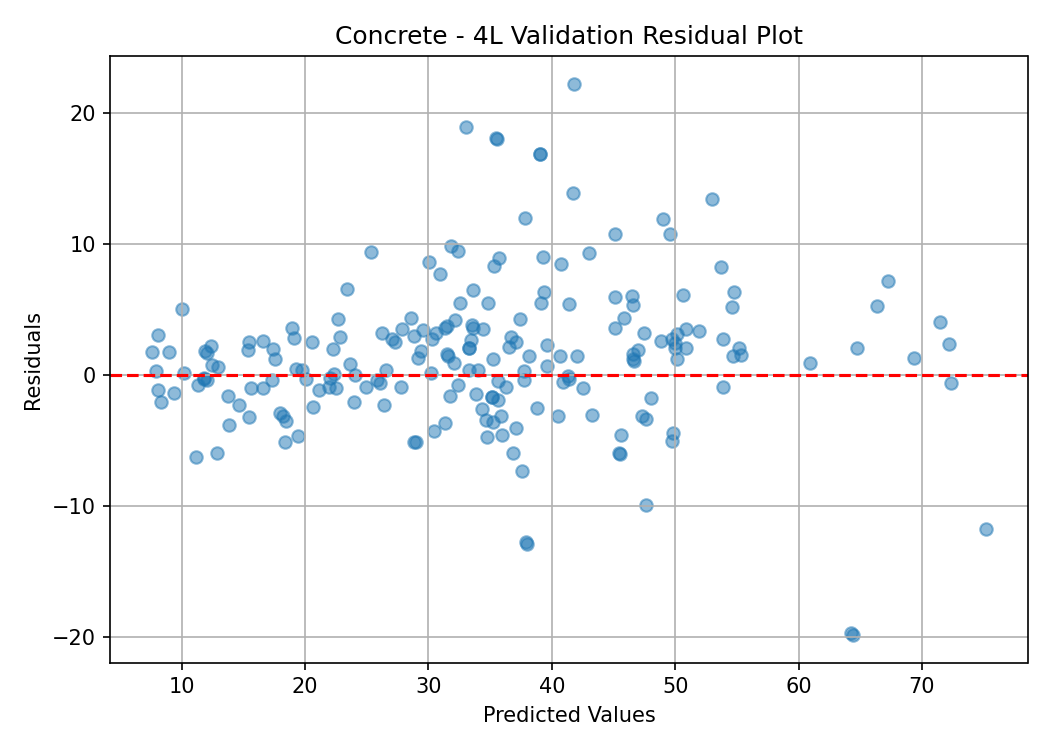
\includegraphics[width=\linewidth]{4L/concrete_residual.png}
        \small (c) Concrete
    \end{minipage}

    \caption{PyTorch 4L Neural Network Validation Residual Plots}
    \label{fig:pytorch4l_residual}
\end{figure}

Figure \ref{fig:pytorch4l_residual} shows the validation residual plots for the three datasets. Airfoil's residuals are small (mostly within $\pm$3 dB) and show no clear pattern, indicating that the hidden layers capture the nonlinear structure that the 2L model missed (its validation RMSE drops from 4.73 to 1.34 dB). However, about 71\% of the Airfoil residuals are positive, indicating that the model slightly underestimates sound pressure on the validation set. Auto MPG's residuals are mostly within $\pm$4 mpg, and the curved pattern seen in the 2L residuals (Figure \ref{fig:pytorch_residual}) is no longer present. Concrete's residuals are centered around zero but spread more widely at mid-range predicted values, with a few large errors near $\pm$20 MPa. All three models have a small positive mean validation residual (0.56 dB, 0.55 mpg, and 1.43 MPa), so they tend to slightly underpredict on unseen data. The Concrete dataset also contains 34 rows with duplicated predictor values, so a small number of validation rows have an identical input in the training set; this affects the 2L and 4L models equally.

\subsection{Comparison with the 2L Neural Network}
\begin{table}[H]
    \centering
    \caption{PyTorch 2L vs. 4L Neural Network Validation $R^2$}
    \label{tab:pytorch_2l_vs_4l}
    \begin{tabular}{lccc}
        \hline
        \textbf{Dataset} & \textbf{2L Validation $R^2$} & \textbf{4L Validation $R^2$} & \textbf{Improvement} \\
        \hline
        Airfoil  & 0.5528 & 0.9643 & +0.4115 \\
        Auto MPG & 0.7829 & 0.8317 & +0.0488 \\
        Concrete & 0.6236 & 0.8691 & +0.2455 \\
        \hline
    \end{tabular}
\end{table}

Table \ref{tab:pytorch_2l_vs_4l} compares the validation R² of the PyTorch 2L and 4L models, which use identical training and validation splits. The 4L model improved validation R² on all three datasets. The largest improvement was for Airfoil (+0.41), whose relationship between frequency, boundary layer thickness, and sound pressure is strongly nonlinear and cannot be captured by the 2L model's linear prediction. Concrete also improved substantially (+0.25), as compressive strength depends nonlinearly on ingredient ratios and curing age. Auto MPG improved the least (+0.05), since a linear model already explains most of its variation. These results also change the ranking of the datasets: Auto MPG had the highest validation R² with the 2L model, but it has the lowest with the 4L model.

\subsection{Conclusion}
Overall, adding two hidden layers greatly improved predictive performance compared with the 2L Neural Network, raising validation R² from 0.55 to 0.96 for Airfoil and from 0.62 to 0.87 for Concrete. The improvement depends on how nonlinear each dataset is: Airfoil and Concrete benefited the most, while Auto MPG, which is close to linear, improved only slightly. The added flexibility also increased the risk of overfitting, most visibly for Concrete, where the training R² (0.96) exceeds the validation R² (0.87). Hyperparameter tuning showed that the best settings vary by dataset, with ReLU and larger hidden layers working best for the two larger datasets. Early stopping was important for controlling overfitting, especially for the small Auto MPG dataset.

